\chapter{Настройка и обслуживание \ReplicaNextLong{}}\label{ch:replica-next-setup-ru}

Настоящий раздел относится к приборной панели \ReplicaNextLong{}, показанной на \autoref{fig:next-hardware-ru}.

\begin{figure}[htbp]
    \centering
    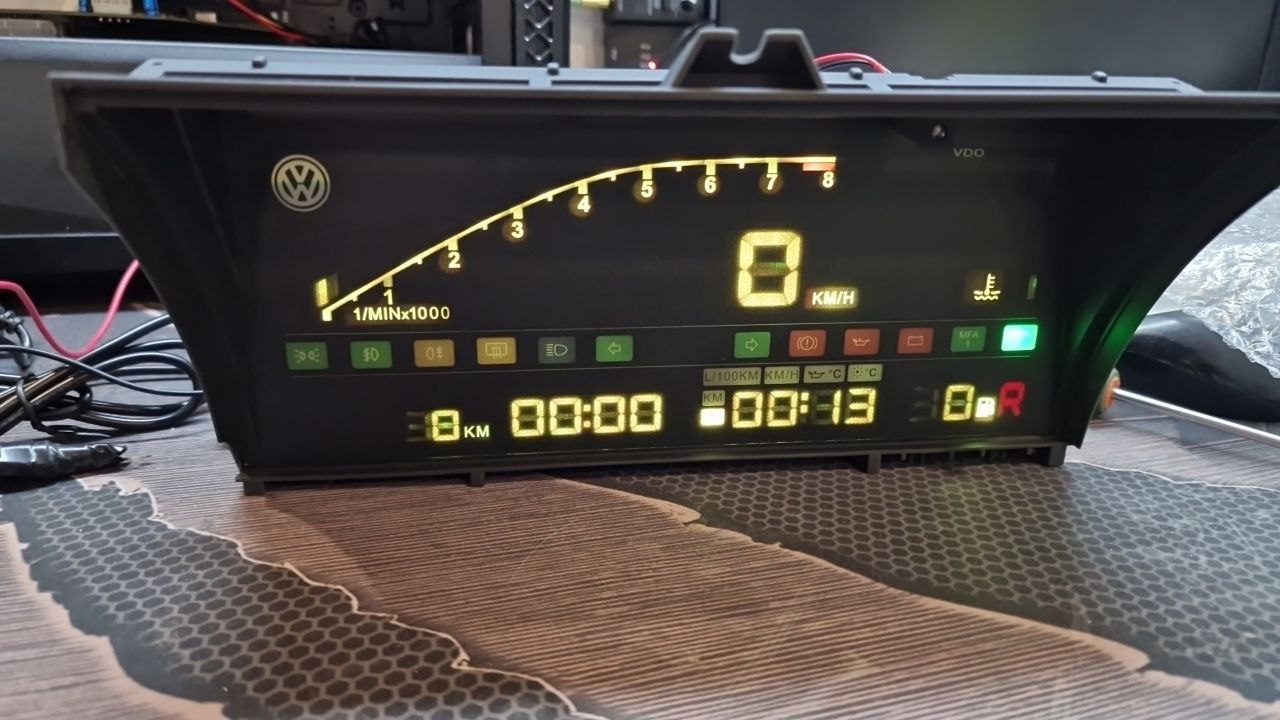
\includegraphics[width=0.6\textwidth]{digifiz_manual/image019.png}
    \caption{Приборная панель \ReplicaNextLong{}.}
    \label{fig:next-hardware-ru}
\end{figure}

\section{Обращение с панелью}
\begin{itemize}
    \item Поликарбонатная лицевую панель с УФ-печатью необходимо защищать от царапин и посторонних предметов. Серьёзные повреждения требуют замены деталей у PHOL-LABS Kft и не рассматриваются как гарантийный случай.
    \item Часы реального времени настраиваются через Wi-Fi-портал управления. При отключении постоянного питания настройки сбрасываются.
\end{itemize}

\section{Веб-портал Wi-Fi}
Конфигурация, сбор данных и управление прошивкой выполняются через встроенное веб-приложение.
\begin{itemize}
    \item Подключитесь к точке доступа приборной панели. Отключите мобильный интернет и подключитесь к сети \texttt{Digifiz\_AP} (пароль \texttt{87654321}); в некоторых версиях используется SSID \texttt{PHOL-LABS2} с тем же паролем.
    \item Адрес по умолчанию — \texttt{192.168.4.1}. Если приборка настроена на подключение к другой сети, просканируйте подсеть с помощью сетевых инструментов и найдите адрес, оканчивающийся на \texttt{.32}.
    \item Портал содержит пять вкладок: \emph{WiFi}, \emph{Control}, \emph{Settings}, \emph{Colors} и \emph{About} (\autoref{fig:next-control-tabs-ru}). Вкладка WiFi отвечает за настройки сети и обновление прошивки; Control регулирует параметры панели; Settings предоставляет структурированный редактор всех параметров прошивки; Colors управляет цветовыми схемами; About содержит сведения об авторе.
\end{itemize}

\begin{figure}[htbp]
    \centering
    \begin{subfigure}{0.48\textwidth}
        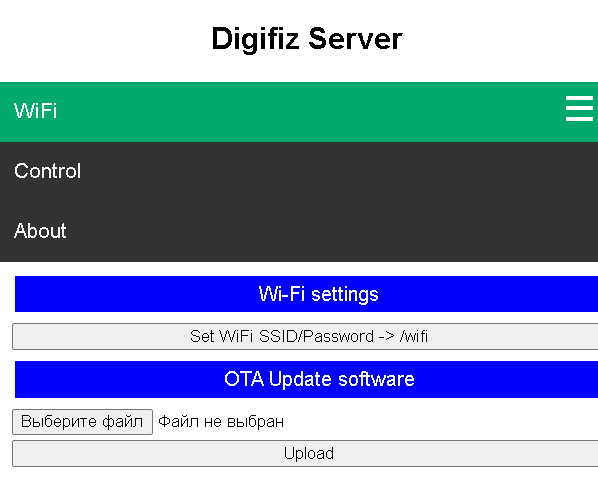
\includegraphics[width=\linewidth]{digifiz_manual/image020.png}
        \caption{Обзор вкладки Control.}
    \end{subfigure}\hfill
    \begin{subfigure}{0.48\textwidth}
        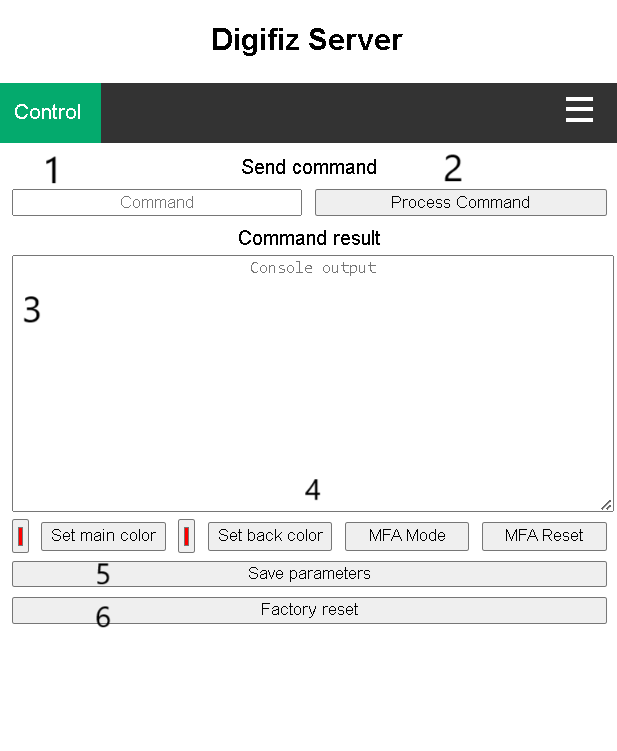
\includegraphics[width=\linewidth]{digifiz_manual/image021.png}
        \caption{Пронумерованные элементы управления и поля ввода команд.}
    \end{subfigure}
    \caption{Wi-Fi интерфейс \ReplicaNextShort{}.}
    \label{fig:next-control-tabs-ru}
\end{figure}

\section{Ввод команд}
На вкладке \emph{Control} доступны строка ввода команд (1), кнопка \emph{Process} (2), окно результатов (3), быстрые переключатели (4), кнопка \emph{Save} (5) и кнопка \emph{Reset} (6).
Команды вводятся в виде пар \verb|<номер> <значение>|, разделённых пробелом; используйте только целые числа, пунктуация не требуется.
\autoref{fig:next-command-example-ru} показывает интерфейс при переключении автоматической регулировки яркости.

\begin{figure}[htbp]
    \centering
    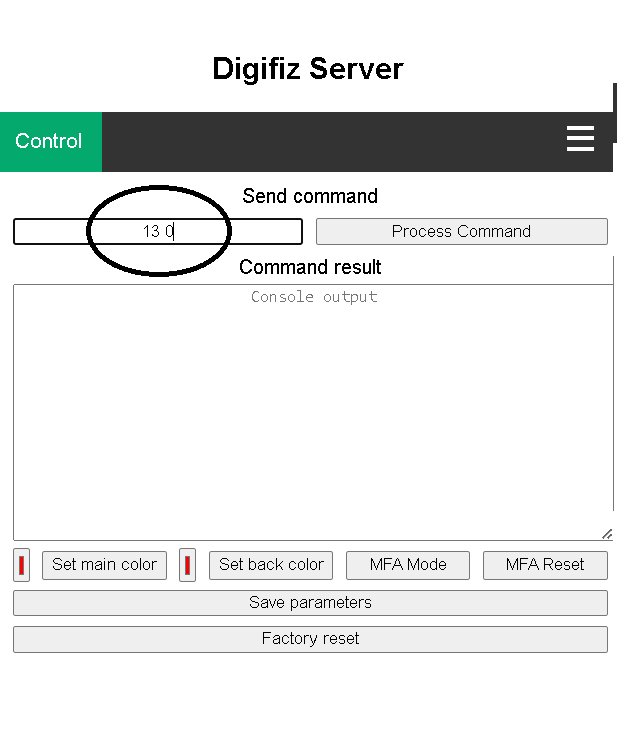
\includegraphics[width=0.55\textwidth]{digifiz_manual/image022.png}
    \caption{Пример команды, отключающей автоматическую яркость.}
    \label{fig:next-command-example-ru}
\end{figure}

\section{Справочник команд}
\begin{table}[htbp]
    \centering
    \caption{Основные команды конфигурации \ReplicaNextShort{}.}
    \label{tbl:next-commands-ru}
    {\scriptsize
    \begin{tblr}{
        colspec = {Q[c,0.14\linewidth] Q[l,0.36\linewidth] Q[l]},
        rowsep = 2pt,
    }
        \toprule
        \textbf{Команда} & \textbf{Название} & \textbf{Описание} \\
        \midrule
        22 (или 0) & \paramname{PARAMETER\_RPMCOEFFICIENT} & Калибровочный коэффициент оборотов двигателя (100--10000). \\
        1  & \paramname{PARAMETER\_SPEEDCOEFFICIENT} & Калибровка скорости (10--255). \\
        2  & \paramname{PARAMETER\_COOLANTTHERMISTORB} & Бета-коэффициент датчика ОЖ (2000--5000). \\
        3  & \paramname{PARAMETER\_OILTHERMISTORB} & Бета-коэффициент датчика температуры масла (2000--5000). \\
        4  & \paramname{PARAMETER\_AIRTHERMISTORB} & Бета-коэффициент датчика наружной температуры (2000--5000). \\
        5  & \paramname{PARAMETER\_TANKMINRESISTANCE} & Минимальное сопротивление датчика уровня топлива (0--1000~\ohm). \\
        6  & \paramname{PARAMETER\_TANKMAXRESISTANCE} & Максимальное сопротивление датчика уровня топлива (100--1000~\ohm). \\
        7  & \paramname{PARAMETER\_TAU\_COOLANT} & Постоянная фильтра температуры ОЖ (1--50, большее значение — быстрее реакция). \\
        8  & \paramname{PARAMETER\_TAU\_OIL} & Постоянная фильтра температуры масла (1--50). \\
        9  & \paramname{PARAMETER\_TAU\_AIR} & Постоянная фильтра наружной температуры (1--50). \\
        10 & \paramname{PARAMETER\_TAU\_TANK} & Постоянная фильтра уровня топлива (1--50). \\
        11 & \paramname{PARAMETER\_MILEAGE} & Суммарный пробег (0--999999). \\
        12 & \paramname{PARAMETER\_DAILY\_MILEAGE} & Суточный пробег (0--9999). \\
        13 & \paramname{PARAMETER\_AUTO\_BRIGHTNESS} & Автоматическая яркость (1 — включена, 0 — выключена). \\
        14 & \paramname{PARAMETER\_BRIGHTNESS\_LEVEL} & Уровень ручной яркости (0--60~\%; значения выше 60 снижают ресурс светодиодов). \\
        15 & \paramname{PARAMETER\_TANK\_CAPACITY} & Ёмкость топливного бака в литрах (0--99; для Golf~2 типично 55~л). \\
        16 & \paramname{PARAMETER\_MFA\_STATE} & Активная страница MFA (обычно управляется аппаратно). \\
        17 & \paramname{PARAMETER\_BUZZER\_OFF} & Отключение зуммера (1 — выключен, 0 — включён; у \ReplicaNextShort{} зуммер отсутствует). \\
        18 & \paramname{PARAMETER\_MAX\_RPM} & Диапазон тахометра (обычно 8000, доступно 4000--16000). \\
        19 & \paramname{PARAMETER\_NORMAL\_RESISTANCE\_COOLANT} & Сопротивление датчика ОЖ при \SI{25}{\celsius} (1000--10000~\ohm). \\
        20 & \paramname{PARAMETER\_NORMAL\_RESISTANCE\_OIL} & Сопротивление датчика масла при \SI{25}{\celsius} (1000--10000~\ohm). \\
        21 & \paramname{PARAMETER\_NORMAL\_RESISTANCE\_AMB} & Сопротивление датчика наружного воздуха при \SI{25}{\celsius} (1000--10000~\ohm). \\
        23 & \paramname{PARAMETER\_DOT\_OFF} & Поведение разделителя часов (0 — мигает, 1 — постоянно). \\
        24 & \paramname{PARAMETER\_BACKLIGHT\_ON} & Включение подсветки при ближнем свете (не используется в \ReplicaNextShort{}). \\
        25 & \paramname{PARAMETER\_M\_D\_FILTER} & Константа медианного фильтра (устаревший параметр). \\
        26 & \paramname{PARAMETER\_COOLANT\_MAX\_R} & Порог датчика ОЖ для полного шкалирования (\SI{100}{\celsius}--\SI{150}{\celsius}). \\
        27 & \paramname{PARAMETER\_COOLANT\_MIN\_R} & Порог датчика ОЖ для индикации «1~bar» (\SI{0}{\celsius}--\SI{80}{\celsius}). \\
        31 & \paramname{PARAMETER\_MAINCOLOR\_R} & Красная компонента цвета интерфейса (0--255). \\
        32 & \paramname{PARAMETER\_MAINCOLOR\_G} & Зелёная компонента цвета интерфейса (0--255). \\
        33 & \paramname{PARAMETER\_MAINCOLOR\_B} & Синяя компонента цвета интерфейса (0--255). \\
        37 & \paramname{PARAMETER\_RPM\_FILTER} & Степень фильтрации оборотов (10--200, большее значение — быстрее реакция). \\
        128 & \paramname{PARAMETER\_READ\_ADDITION} & Добавьте 128, чтобы считать текущее значение любой команды. \\
        255 & \paramname{PARAMETER\_SET\_HOUR} & Установка часов (24-часовой формат). \\
        254 & \paramname{PARAMETER\_SET\_MINUTE} & Установка минут. \\
        253 & \paramname{PARAMETER\_RESET\_DAILY\_MILEAGE} & Сброс суточного пробега. \\
        252 & \paramname{PARAMETER\_RESET\_DIGITAL} & Заводской сброс сохранённых параметров. \\
        \bottomrule
    \end{tblr}}
\end{table}

\section{Значения по умолчанию}
\begin{table}[htbp]
    \centering
    \caption{Заводские настройки \ReplicaNextShort{}.}
    \label{tbl:next-defaults-ru}
    {\scriptsize
    \begin{tblr}{
        colspec = {Q[l,0.42\linewidth] Q[c,0.15\linewidth] Q[l]},
        rowsep = 2pt,
    }
        \toprule
        \textbf{Параметр} & \textbf{Значение} & \textbf{Примечание} \\
        \midrule
        \paramname{PARAMETER\_RPMCOEFFICIENT} & 3000 & Типично для входов тахометра Audi. \\
        \paramname{PARAMETER\_SPEEDCOEFFICIENT} & 100 & Калибровано на 100~км/ч. \\
        \paramname{PARAMETER\_COOLANTTHERMISTORB} & 4000 &  \\
        \paramname{PARAMETER\_OILTHERMISTORB} & 4000 &  \\
        \paramname{PARAMETER\_AIRTHERMISTORB} & 3812 & Для панелей поколения~2 — 3600. \\
        \paramname{PARAMETER\_TANKMINRESISTANCE} & 35 & \ohm. \\
        \paramname{PARAMETER\_TANKMAXRESISTANCE} & 265 & \ohm. \\
        \paramname{PARAMETER\_TAU\_COOLANT} & 2 & Константа фильтра. \\
        \paramname{PARAMETER\_TAU\_OIL} & 2 & Константа фильтра. \\
        \paramname{PARAMETER\_TAU\_AIR} & 2 & Константа фильтра. \\
        \paramname{PARAMETER\_TAU\_TANK} & 2 & Константа фильтра. \\
        \paramname{PARAMETER\_MILEAGE} & Зависит от автомобиля & Сохраняет текущий пробег. \\
        \paramname{PARAMETER\_DAILY\_MILEAGE} & 0 &  \\
        \paramname{PARAMETER\_AUTO\_BRIGHTNESS} & 1 & Включена. \\
        \paramname{PARAMETER\_BRIGHTNESS\_LEVEL} & 25 & Значение по умолчанию для поколения~2; для поколений~1/1.5 — 7 или 13. \\
        \paramname{PARAMETER\_TANK\_CAPACITY} & 63 & Литры. \\
        \paramname{PARAMETER\_MFA\_STATE} & 0 & Страница MFA по умолчанию. \\
        \paramname{PARAMETER\_BUZZER\_OFF} & 1 & Зуммер отключён. \\
        \paramname{PARAMETER\_MAX\_RPM} & 8000 & Диапазон тахометра. \\
        \paramname{PARAMETER\_NORMAL\_RESISTANCE\_COOLANT} & 1000 & \ohm{} при \SI{25}{\celsius}. \\
        \paramname{PARAMETER\_NORMAL\_RESISTANCE\_OIL} & 1000 & \ohm{} при \SI{25}{\celsius}. \\
        \paramname{PARAMETER\_NORMAL\_RESISTANCE\_AMB} & 2991 & Для датчиков поколения~2 — 500~\ohm. \\
        \paramname{PARAMETER\_DOT\_OFF} & 0 & Мигающий разделитель времени. \\
        \paramname{PARAMETER\_BACKLIGHT\_ON} & 1 & Подсветка включается с ближним светом. \\
        \paramname{PARAMETER\_M\_D\_FILTER} & 65535 & Константа медианного фильтра. \\
        \paramname{PARAMETER\_COOLANT\_MAX\_R} & 120 & \si{\celsius}. \\
        \paramname{PARAMETER\_COOLANT\_MIN\_R} & 60 & \si{\celsius}. \\
        \paramname{PARAMETER\_MAINCOLOR\_R} & 180 & Базовый жёлто-зелёный оттенок. \\
        \paramname{PARAMETER\_MAINCOLOR\_G} & 240 & Базовый жёлто-зелёный оттенок. \\
        \paramname{PARAMETER\_MAINCOLOR\_B} & 6 & Базовый жёлто-зелёный оттенок. \\
        \paramname{PARAMETER\_RPM\_FILTER} & 70 & Реакция фильтра. \\
        \paramname{PARAMETER\_UPTIME} & 0 & Счётчик времени работы. \\
        \bottomrule
    \end{tblr}}
\end{table}

\section{Чтение параметров и примеры}
Чтобы считать параметр, прибавьте 128 к номеру команды (например, \verb|129 0| выводит коэффициент скорости).
Типичные команды: отключение автоматической яркости (\verb|13 0|), повторное включение (\verb|13 1|), корректировка коэффициента скорости (\verb|1 110| увеличивает показания на 10~\%), установка одометра (\verb|11 123456|).
Значения часов задаются последовательностью \verb|255 <часы>| и \verb|254 <минуты>|.
Команды 31--33 задают RGB-компоненты пользовательского цвета интерфейса.

\section{Сервисные команды}
В свежих версиях прошивки поддерживается ввод понятных имен параметров, например \verb|PARAMETER_RPMCOEFFICIENT 3000|.
Диагностическая команда \verb|adc 0| выводит сырые значения АЦП для проверки датчиков.
Обновления прошивки добавляют визуальные настройки цветов, поэтому рекомендуется регулярно устанавливать их через вкладку \emph{WiFi}.

\section{Редактор параметров во вкладке Settings}
Вкладка \emph{Settings} повторяет список параметров из \autoref{tbl:next-commands-ru} и \autoref{tbl:next-defaults-ru}, дополняя его метаданными о диапазонах, описаниях и типах данных.
Используйте её, если предпочитаете графический интерфейс вместо ввода числовых команд.
